% Config
\documentclass{beamer}
\usepackage[utf8]{inputenc}

% Packages
\usepackage{multicol}
\usepackage[francais]{babel}
\usepackage{amsfonts, amsthm, amssymb, amsmath}
\usepackage{xcolor}
\usepackage{mathtools}
\usepackage{ninecolors}
\usepackage{physics}
\usepackage{hyperref}
\usepackage{adjustbox}
\usepackage{listings}

\hypersetup{colorlinks=true, linkcolor=black, urlcolor=black}

\title{TP5 Thermodynamique}
\author{BERREDO DE LA COLINA Lucas\\ MARTIN Lola}
\date{}

\usetheme[nofirafonts]{focus}

\lstset{frame=tb,
  language=Python,
  aboveskip=3mm,
  belowskip=3mm,
  showstringspaces=false,
  columns=flexible,
  basicstyle={\small\ttfamily},
  numbers=none,
  numberstyle=\tiny\color{gray},
  keywordstyle=\color{blue},
  commentstyle=\color{darkgreen}, 
  stringstyle=\color{mauve},
  breaklines=true,
  breakatwhitespace=true,
  tabsize=4
}

% Commands
\newcommand{\newlines}{\newline\newline}



% Document
\begin{document}




\begin{frame}
\vfill
\Huge{TP5 Thermodynamique}

\Large{Partie 1: Rayonnement}
\\[2em]
\large{BERREDO DE LA COLINA Lucas\\ MARTIN Lola}
\\[2em]
{\small Fichiers: \url{https://github.com/LucasBerredo/DiapoThermo}}

\end{frame}





\begin{frame}
\frametitle{But de l'experience}

\begin{itemize}
	\item{L'emissivité}
    

    Nous allons determiner l'emmissivité d'un corps noir et gris.

    Pour cela nous avons:
    \[
    \epsilon = \frac{C}{\tau S_1 \sigma 4 T_f^3}
    \]

    \item{Échange de chaleur}

    
    Nous allons déterminer l'échange de chaleur de nos deux corps
    
    $h$ représente l'ensemble des échanges de chaleur (conduction,rayonement,convection)
    \[
    h= \frac{C}{\tau' S_1}-\frac{\sigma 4 T_f^3}{\frac{1}{\epsilon}+\frac{1}{\epsilon_{air}}-1}
    \]

\end{itemize}

\end{frame}





\begin{frame}
\frametitle{Explication de l'expérience}

\begin{itemize}
    \item La variation de température obéit à l'équation différentielle :

    \[
    C \frac{dT}{dt} = \epsilon S \sigma \left( T_f^4 - T(t)^4 \right)
    \]

    \item Résolution exacte :

    \[
    \scalebox{0.62}{
    $\displaystyle
    t = 2\tau \left[
    \left( \arctan\left( \exp\left( 2 \tanh^{-1} \frac{T(t)}{T_f} \right) \right)
    - \arctan\left( \exp\left( 2 \tanh^{-1} \frac{T_i}{T_f} \right) \right) \right)
    + \left( \tanh^{-1} \frac{T(t)}{T_f} - \tanh^{-1} \frac{T_i}{T_f} \right)
    \right]
    $}
    \]

    \item Résolution approchée :

    \[
    T = T_f + (T_i - T_f) \left( 1 - \exp\left( \frac{-t}{\tau} \right) \right)
    \]

\end{itemize}
\end{frame}

\begin{frame}
\frametitle{Explication de l'expérience}

\begin{itemize}
    \item Mise sous vide :

    Évite les échanges de chaleur ($h = 0$)

    \item Pression ambiante :

    Permet de mesurer l’échange de chaleur
\end{itemize}

\end{frame}



\begin{frame}
\frametitle{Dispositif expérimental}

\begin{itemize}
	\item{Deux échantillons (gris, noir)\newline}
	\item{Deux chambres:\newline
	\begin{itemize}
		\item{Four ($200^{\circ}C$)\newline}
		\item{Refroidessement à l'eau\newline}
	\end{itemize}}
	\item{Elles peuvent être mises sous vide\newline}
	\item{Mesures de temperature analogiques (100 points, 15 min)}
\end{itemize}
\end{frame}





\begin{frame}
\frametitle{Experiences}

\begin{enumerate}
	\item{{\color{gray7}Corps gris}{\color{gray4}, {\color{red}chauffage}, vide}\newline}
	\item{{\color{gray7}Corps gris}{\color{gray4}, {\color{blue5}refroidissement}, vide}\newline}
	\item{{\color{gray7}Corps gris}{\color{gray4}, {\color{red}chauffage}, sans vide}\newline}
	\item{{\color{gray7}Corps gris}{\color{gray4}, {\color{blue5}refroidissement}, sans vide}\newline}
	\item{{\color{black}Corps noir}{\color{gray4}, {\color{red}chauffage}, vide}\newline}
	\item{{\color{black}Corps noir}{\color{gray4}, {\color{red}chauffage}, sans vide}\newline}

\end{enumerate}
\end{frame}





\begin{frame}
\frametitle{Organisation des données}

\centering
\begin{minipage}{0.48\textwidth}
    \centering
    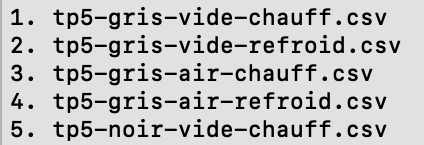
\includegraphics[width=\linewidth]{Fig/ls-csv.png}
\end{minipage}
\hfill
\begin{minipage}{0.48\textwidth}
    \centering
    \adjustbox{valign=c}{
        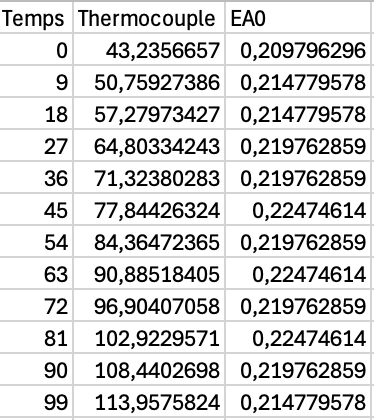
\includegraphics[width=\linewidth]{Fig/example-csv.png}}
\end{minipage}
\end{frame}





\begin{frame}
\frametitle{Approximation graphique 1er ordre}

Il ne faut que vérifier les valeur initiales, finales et approcher $\tau$ de façon qu'on trouve des courbes proches

\begin{figure}
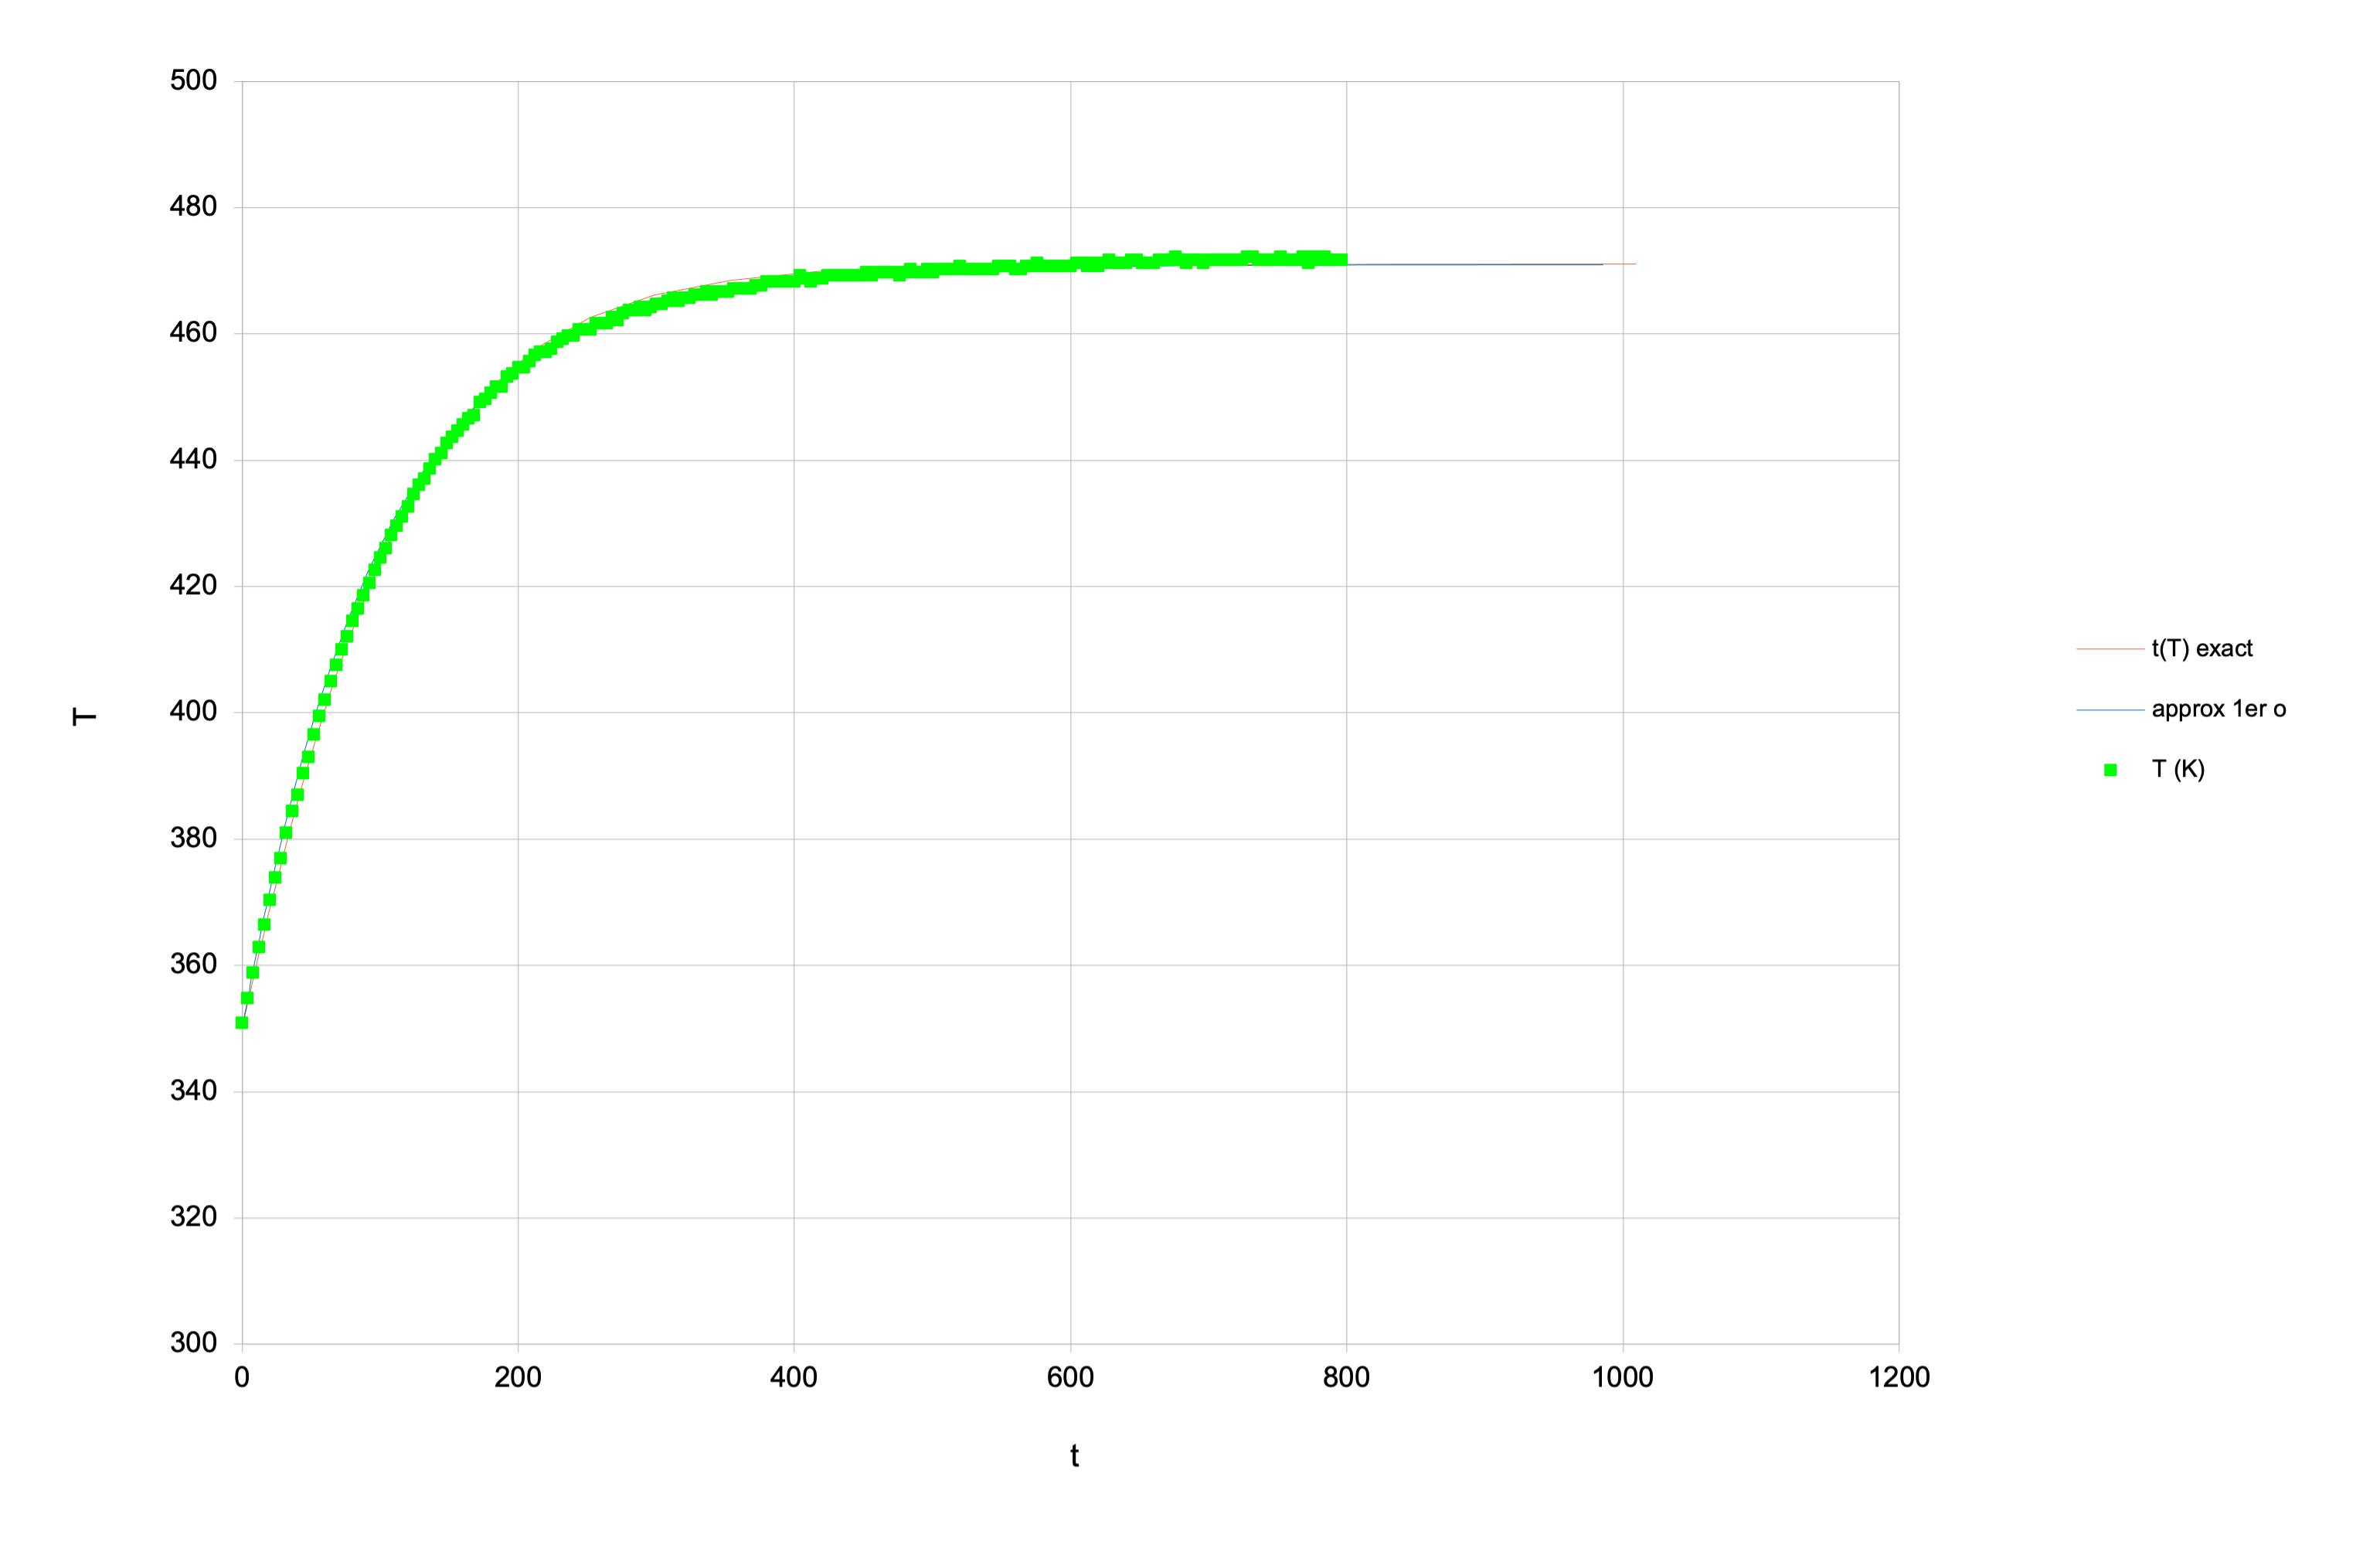
\includegraphics[width=0.75\textwidth]{Fig/t1-100-t2-82.png}
\caption{Example representation graphique: Vert: points experimentaux, Bleu: courbe théorique}
\end{figure}

\end{frame}





\begin{frame}
\frametitle{Approximation graphique}

Nous obtenons les prochains valeurs:
\begin{enumerate}
	\item{{\color{gray7}Corps gris}{\color{gray4}, {\color{red}chauffage}, vide} \hfill $\tau = 100$\hspace{4em} \newline}
	\item{{\color{gray7}Corps gris}{\color{gray4}, {\color{blue5}refroidissement}, vide} \hfill $\tau = 69$\hspace{4em} \newline}
	\item{{\color{gray7}Corps gris}{\color{gray4}, {\color{red}chauffage}, sans vide} \hfill $\tau = 117$\hspace{4em} \newline}
	\item{{\color{gray7}Corps gris}{\color{gray4}, {\color{blue5}refroidissement}, sans vide} \hfill $\tau = 68$\hspace{4em} \newline}
	\item{{\color{black}Corps noir}{\color{gray4}, {\color{red}chauffage}, vide} \hfill $\tau = 105$\hspace{4em} \newline}
	\item{{\color{black}Corps noir}{\color{gray4}, {\color{red}chauffage}, sans vide}\hfill $\tau = 99$\hspace{4em} \newline}
\end{enumerate}
\end{frame}





\begin{frame}
\frametitle{Approximation graphique 2ème ordre}
\begin{enumerate}
	\item{{\color{gray7}Corps gris}{\color{gray4}, {\color{red}chauffage}, vide} \hfill $\tau = 82$\hspace{4em} \newline}
	\item{{\color{gray7}Corps gris}{\color{gray4}, {\color{blue5}refroidissement}, vide} \hfill $\tau = 85$\hspace{4em} \newline}
	\item{{\color{gray7}Corps gris}{\color{gray4}, {\color{red}chauffage}, sans vide} \hfill $\tau = 100$\hspace{4em} \newline}
	\item{{\color{gray7}Corps gris}{\color{gray4}, {\color{blue5}refroidissement}, sans vide} \hfill $\tau = 84$\hspace{4em} \newline}
	\item{{\color{black}Corps noir}{\color{gray4}, {\color{red}chauffage}, vide} \hfill $\tau = 111$\hspace{4em} \newline}
	\item{{\color{black}Corps noir}{\color{gray4}, {\color{red}chauffage}, sans vide}\hfill $\tau = 89$\hspace{4em} \newline}
\end{enumerate}

\end{frame}





\begin{frame}
\frametitle{Approximation numérique avec Python}
Comme nous avons la résolution pour $\tau$, nous pouvons donner ça vers un $\texttt{curve\_fit}$ dans Python.

\begin{figure}
\includegraphics[width=\textwidth]{Fig/Python_Refroid.png}
\caption{Exemple refroidissement. Il y a aussi un fichier pour chauffement.}
\end{figure}

\end{frame}





\begin{frame}
\frametitle{Approximation numérique avec Python}
Résultats:
\begin{enumerate}
	\item{{\color{gray7}Corps gris}{\color{gray4}, {\color{red}chauffage}, vide} \hfill $\tau = 96,0399...$\hspace{4em} \newline}
	\item{{\color{gray7}Corps gris}{\color{gray4}, {\color{blue5}refroidissement}, vide} \hfill $\tau = 86,1429...$\hspace{4em} \newline}
	\item{{\color{gray7}Corps gris}{\color{gray4}, {\color{red}chauffage}, sans vide} \hfill $\tau = 99,2634...$\hspace{4em} \newline}
	\item{{\color{gray7}Corps gris}{\color{gray4}, {\color{blue5}refroidissement}, sans vide} \hfill $\tau = 84,5618...$\hspace{4em} \newline}
	\item{{\color{black}Corps noir}{\color{gray4}, {\color{red}chauffage}, vide} \hfill $\tau = 111,8591...$\hspace{4em} \newline}
	\item{{\color{black}Corps noir}{\color{gray4}, {\color{red}chauffage}, sans vide}\hfill $\tau = 90,5110...$\hspace{4em} \newline}
\end{enumerate}
\end{frame}





\begin{frame}
\frametitle{Comparaison des résultats}

\begin{table}[htdp]\begin{center}\begin{tabular}{|c|c|c|c|}
\hline
Expérience & 1er ordre & 2ème ordre & Python \\
\hline
1 & 100 & 82 & 96,0399 \\
2 & 69 & 85 & 86,1429 \\
3 & 117 & 100 & 99,2634 \\
4 & 68 & 84 & 84,5618 \\
5 & 105 & 111 & 111,8591 \\
6 & 99 & 89 & 90,5110 \\
\hline
\end{tabular} 
\caption{Valeurs du paramètre $\tau$}\end{center}\label{defaulttable}\end{table}

\end{frame}





\begin{frame}
\frametitle{Analyse des résultats}

\begin{itemize}
	\item{Les valeurs generés par Python suivent avec le moindre erreur possible la courbe.\newline}
	\item{L'approximation à premier ordre a un erreur autour 20\% pour chaque expérience.\newline}
	\item{L'approximation à deuxième ordre est beaucoup plus proche (autour $\pm1$ point).\newline}
\end{itemize}

\end{frame}


\begin{frame}
\frametitle{Analyse des résultats}
On trouve les résultats suivant
\begin{itemize}
	\item{$\epsilon_{gris}=0,54 $\newline}

	\item{$h_{gris}=11,27 W.m.K^{-1} $\newline}
    \item{$\epsilon_{noir}=0,76 $\newline}
    \item{$h_{noir}=15,13 W.m.K^{-1} $\newline}
\end{itemize}

\end{frame}




\begin{frame}
\vfill
\Huge{TP5 Thermodynamique}

\Large{Partie 2: Loi de Stefan}
\\[2em]
\large{BERREDO DE LA COLINA Lucas\\ MARTIN Lola}
\\[2em]
{\small Fichiers: \url{https://github.com/LucasBerredo/DiapoThermo}}

\end{frame}





\begin{frame}
\frametitle{Avertissement}
Bien que nous ayons travaillé avec l'équipement et observé des résultats avec Mme Quilliet, nous n'avons pas enregistré de résultats numériques.
\end{frame}





\begin{frame}
\frametitle{Rappel théorique}

\begin{itemize}
	\item{ Loi de Stefan}

    \[
    M= \sigma T^4
    \]

    Avec M la densité de puissance ($W.m^{-2})$

\end{itemize}



\begin{figure}
\includegraphics[height=1in]{Fig/shemas.png}
\caption{Shémas de l'experience}
\end{figure}

\end{frame}






\begin{frame}
\frametitle{Dispositif experimental}

\begin{itemize}
	\item{Deux parties:\newline
	\begin{itemize}
		\item{Côté emmisive - Boule à cuivre ``corps noir''\newline}
		\item{Côté receptive - Thermopile CA2 (filtre en option) et multimètre\newlines}
	\end{itemize}}
	\item{Emmisivité fixé - mesure du puissance avec le multimètre\newline}
	\item{Il faut attendre après chaque changement vers la stabilisation\newline}
	\item{Mesures a plusieurs distances (0,3; 0,4; 0,8; 1,2m) et temperatures (20, 60, 90, 120 $^\circ C$)}
	
\end{itemize}	
	
\end{frame}





\begin{frame}
\frametitle{Approximation des résultats}

\begin{figure}
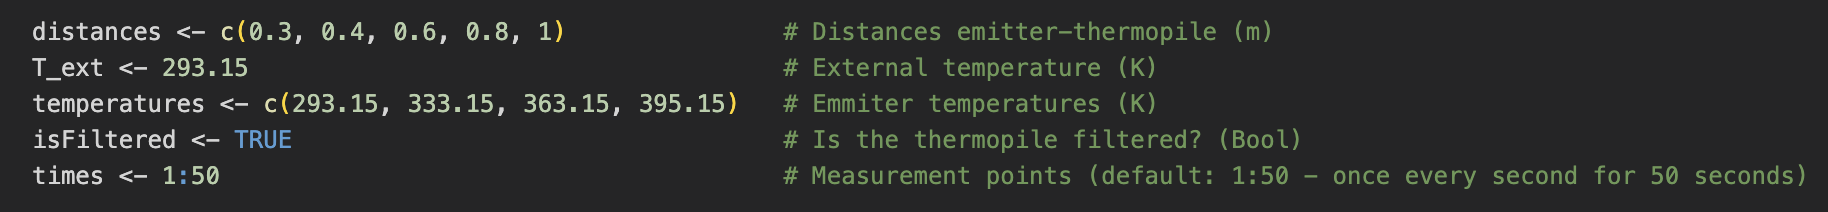
\includegraphics[height=0.5in]{Fig/stefan-params.png}
\caption{Paramètres à choisir}
\end{figure}

\begin{figure}
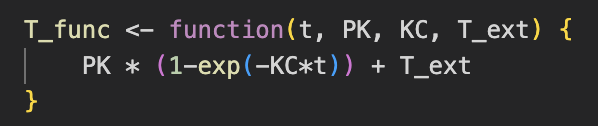
\includegraphics[height=0.5in]{Fig/evol-temporelle.png}
\caption{Fonction pour l'évolution temporelle théorique}
\end{figure}

\end{frame}





\begin{frame}
\frametitle{Approximation des résultats}

\begin{figure}
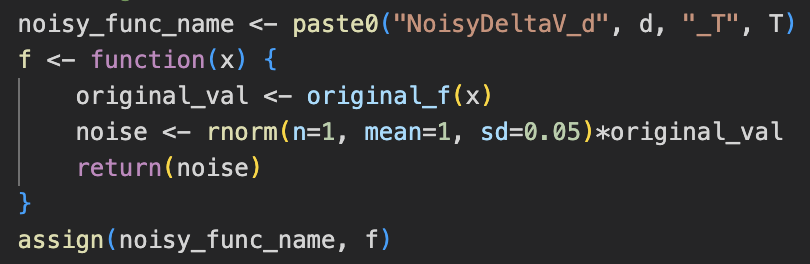
\includegraphics[width=0.75\textwidth]{Fig/bruit.png}
\caption{Ajout du bruit}
\end{figure}

\end{frame}





\begin{frame}
\frametitle{Approximation des résultats}
\centering
\begin{minipage}{0.48\textwidth}
    \centering
    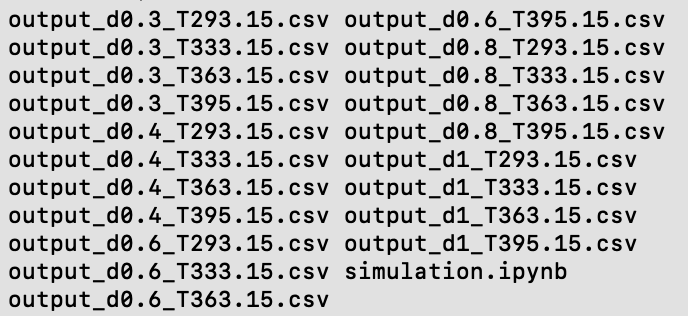
\includegraphics[width=\linewidth]{Fig/stefan-fichiers.png}
    \textbf{Figure} -- Fichiers generés par le script
\end{minipage}
\hfill
\begin{minipage}{0.48\textwidth}
    \centering
    \adjustbox{valign=c}{
        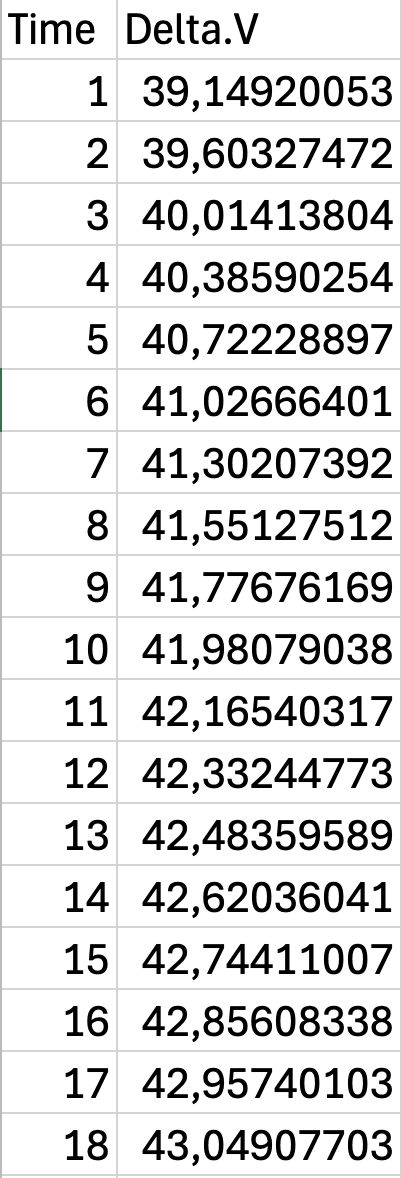
\includegraphics[width=0.4\linewidth]{Fig/stefan-csv.png}}
        
        \textbf{Figure} -- Example des premières colonnes du .csv
\end{minipage}     

\end{frame}



\begin{frame}
\frametitle{Analyse des données}
Pour chaque fichier:
\begin{itemize}
	\item{On attend jusqu'à la courbe est presque stabilisé. (Après 30 secondes).}
	\item{On prend la moyenne des résultats après $t=30$, afin de trouver un résultat plus proche au valeur théorique}
	\item{En utilisant la formule $$\sigma = \frac{U}{\alpha\left(\frac{r}{r+d+d_0}\right)^2 (T^4-T_{ext}^4)},$$ on calcule la constante de Stefan}

\end{itemize}
\end{frame}





\begin{frame}
\frametitle{Analyse des données}
\begin{table}[htdp]\begin{center}
\resizebox{\textwidth}{!}{
\begin{tabular}{|c|ccc|}
\hline
Dist\textbackslash Temp & 333,15 & 363,15 & 395,15 \\
\hline
0,3 & 1,491E-09 (2,63\%)& 1,546E-09 (2,72\%) & 5,364E-09 (9,45\%)\\
0,4 & 4,668E-09 (8,23\%) & 9,580E-11 (0,17\%)& 1,443E-10 (0,25\%)\\
0,6 & 2,277E-09 (4,01\%)& 2,754E-09 (4,85\%)& 1,676E-09 (2,95\%)\\
0,8 & 1,078E-09 (1,90\%)& 1,065E-10 (0,19\%)& 1,200E-09 (2,12\%)\\
1 & 4,995E-10 (0,88\%)& 2,061E-10 (0,36\%)& 4,690E-10 (0,83\%)\\
\hline
\end{tabular}
}
 \caption{Erreur absolue (erreur relative)}\end{center}\label{defaulttable}\end{table}

\end{frame}



\end{document}
